\chapter{Experiments}


\section{Servo Setting Time}

It takes non-trivial time for the steering servo to move from its previous position to a newly set position. The steering angle changes continuously as the servo adjusts and it affects the direction in which the vehicle travels in the meantime. In this experiment, we measure the setting time of the servo between different steering angles and based on the data, we will find a relationship between the distance between the servo position and the time it will take to set.

The position of the servo is set through a \gls{PWM} value between \SI{1200}{\micro\second} (rightmost position), \SI{1500}{\micro\second} (center position), and \SI{1800}{\micro\second} (leftmost position). In this procedure, the vehicle switches between a right position $r$ and a left position $l$ a hundred times while the vehicle is stationary and it is placed on a flat surface. The servo produces a noise during the whole setting period and is mostly quiet during the periods between adjustments.

We record the sound the servo makes through a microphone. The audio track is then edited using \textit{Audacity}\footnote{https://www.audacityteam.org/} to remove background noise and low frequency ``buzzing'' of the servo and to use the ``Sound Finder'' analysis tool to label periods of sound in the cleaned audio track (see Figure~\ref{fig:audacity}). The start and end times of the labeled intervals are then exported into a text file for further analysis.

We carried out this procedure for five pairs of \gls*{PWM} values: $(1800, 1200)$, $(1750, 1250)$, $(1700, 1300)$, $(1650, 1450)$, $(1600, 1400)$. Each of these pairs is symmetrical around the center position \SI{1500}{\micro\second} and the \textit{distance} between the two positions decreases from \SI{600}{\micro\second} to \SI{200}{\micro\second}. This might have biased the results and decrease the accuracy of our result.

\begin{figure}
	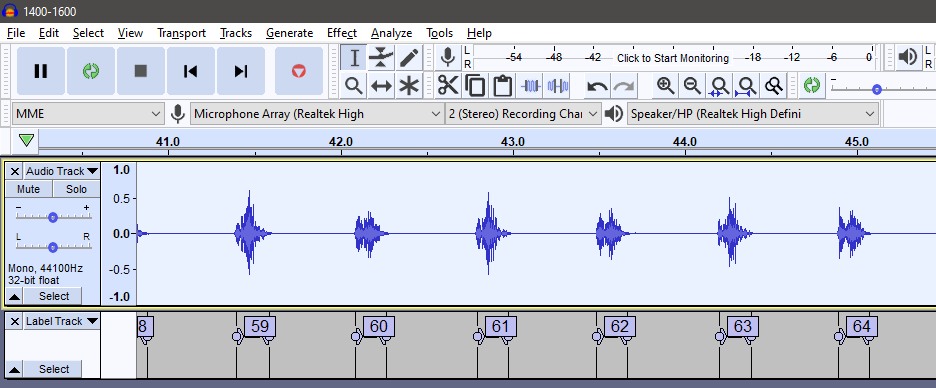
\includegraphics[width=\textwidth]{../img/servo_experiment_audacity}
	\protect\caption{The servo setting periods are clearly identifiable in an audio recording after background noise and low frequency sounds are removed. This figure shows the interface of the \textit{Audacity} tool used to analyze a recording of adjustments between the PWM signal of \SI{1400}{\micro\second} and \SI{1600}{\micro\second}.}
	\label{fig:audacity}
\end{figure}

We used the method of least squares to find a best fitting line in the form of $t=ad+b$, where $t$ is the setting time in seconds and $d$ is the distance between the \gls*{PWM} values. Based on the data we recorded, the relationship between the distance to the new servo position and the setting time is visualized in the Figure~\ref{fig:servo_linear_regression} and in the following equation:

\begin{equation}
	\label{eq:servo_setting_time}
	t=0.000329d + 0.1174.
\end{equation}

\begin{figure}
	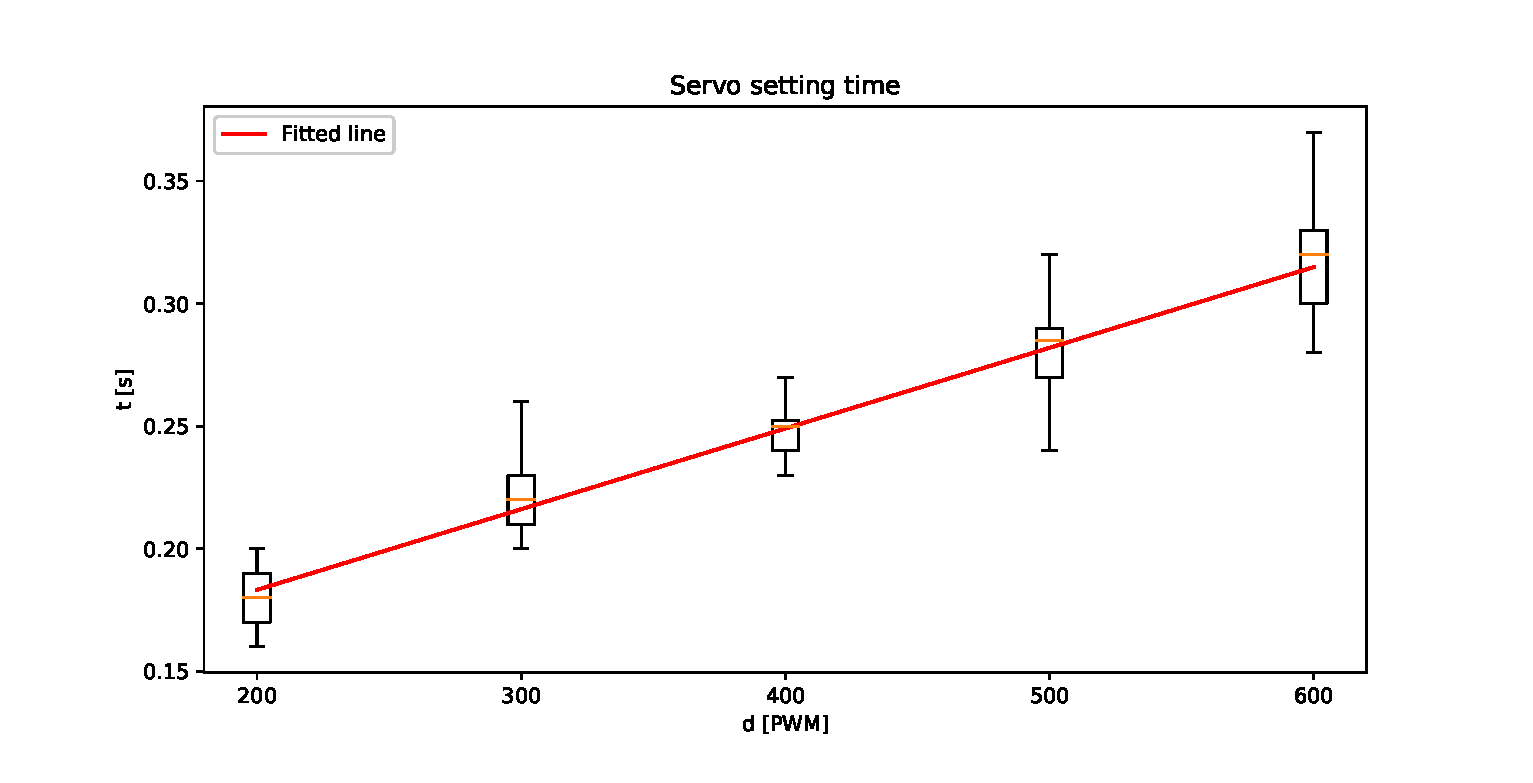
\includegraphics[width=\textwidth]{../img/servo_setting_time_linreg.eps}
	\caption{The setting time of the steering servo can be estimated with a linear function of the distance between the start and end PWM values.}
	\label{fig:servo_linear_regression}
\end{figure}

\section{Motor Shaft Angular Velocity Modeling}